%!TEX root=../mythesis.tex
% Chapter 1

\chapter{Introduction} % Main chapter title
\chaptermark{Introduction}
\label{ch:introduction} % For referencing the chapter elsewhere, use \ref{Chapter1} 
%----------------------------------------------------------------------------------------
%	SECTION 1
%----------------------------------------------------------------------------------------
\section{Motivation and Challenge}
Smart contracts are stateful computer programs running on blockchain platforms to manage large sums of
cryptocurrency, govern and carry out transactions of assets between multiple parties.
The blockchain technology has been booming in recent years, since the introduction of Bitcoin~\cite{nakamoto2008bitcoin} by Nakamoto in 2008.
The blockchain networks can be broadly categorized into the permissionless and permissioned blockchains, where the former is open to the public (e.g.,
Bitcoin~\cite{nakamoto2008bitcoin} and Ethereum~\cite{Ethereum}) and the latter is only accessible to trusted groups or private institutions (e.g., Hyperledger Fabric~\cite{hyperledger-fabric} and FISCO BCOS~\cite{fisco}).
The distributed and tamper-resistant nature of blockchain has made it the perfect platform for hosting smart contracts.
Ethereum~\cite{Ethereum} and EOS~\cite{EOS} are the most popular permissionless blockchain platforms which
support smart contracts applicable in many areas.
As of Nov 2020, there are over 1.5 million smart contracts deployed on Ethereum, which is a 100 fold increase since just two years ago.
These smart contracts have enabled about 3.1K decentralized applications (DApps)~\cite{dapp-stats}
serving around 80K daily users on finance, health, governance, gambling, games, etc.


\textcolor{black}{The security of smart contracts} has attracted great attention, ever since their adoption in the management of massive cryptocurrency transactions.
The most notorious attack is that malicious attackers exploited the \emph{reentrancy vulnerability} in the DAO contract on Ethereum~\cite{DAO_attacks}, which resulted in
a loss of \$60 million worth in 2016.
EOS gambling games were intensively hacked in 2019 using a technique called the \emph{transaction congestion attack}~\cite{EOS_attacks} and led
to significant asset loss of smart contract applications such as \texttt{EOS.WIN} and \texttt{EOSPlay}.
The root cause of these attacks is that certain security vulnerabilities introduced during contract development are exploited by malicious parties, causing a loss for the contract owners (and possibly other honest participants).
Most vulnerabilities subject to programming errors, indicating a mismatch between the contract developers' expectations and how the contract code actually works.
Therefore, much research has been dedicated to preventing attacks, discovering and mitigating such vulnerabilities .

\textcolor{black}{However, little work has been done on more enterprise smart contract applications} for its great complexity.
The contract execution on permissionless chains is bounded by limited resource such that smart contracts are often kept simple.
For example, on Ethereum, user has to pay miners (who in charge of executing transactions) a certain amount of ``gas'' (cryptocurrency on Ethereum) as the transaction fee to deploy or interact with contract, which is mainly decided by the computational complexity of contracts (e.g., up to \$15 in fees~\cite{gas-fee}).
Therefore, most permissionless blockchains are mainly used for crytocurrency exchange (e.g., ERC Token and DeFi applications).
In contrast, the permissioned blockchains aim to create real value.
For instance, FISCO BCOS has been successfully adopted in areas such as government and judicial services, supply chain, finance, health care, copyright management, education, transportation, and agriculture~\cite{fisco}.
The smart contracts powering these enterprise applications are more sophisticated and often demonstrate strong stateful behaviors.
However, existing testing and analysis tools~\cite{jiang2018contractfuzzer,oyente,securify,SmartCheck,wang2019vultron} target only Ethereum smart contracts and mainly focus on their security issues, which will not work well in these stateful enterprise smart contracts due to the lack of understanding of system behaviours, absence of test oracles and missing measurement of test adequacy.
The aforementioned enterprise smart contracts on permissioned blockchains are usually well specified, which make it suitable for model based testing (MBT).
However, as for most smart contracts on permissionless blockchains, system behaviours and requirements are not specified thus making existing MBT tools impractical for finding logic bugs.
Even though, popular Ethereum DApps have attracted many users in thousands or even millions of transactions~\cite{Etherscan} that occurred in the past.
Learning likely specification requirement, e.g, access control model and state machine model is feasible via time travel on transaction history of smart contracts free of attacks in the past.
With likely requirement of contracts, it is easily to facilitate testing or verification to find logic bugs or prove logic property.
 
Compared to the security, \textcolor{black}{the \emph{fairness} issues of smart contracts have not yet attracted much attention}.
Smart contracta are unfair to certain participants if there is a mismatch between the participants' expectations and the actual implementation of the game rules.
Although a malicious party may gain an advantage over others through the exploitation of security vulnerabilities, e.g., examining other participants' actions in a sealed game,
we would like to focus more on the fairness issues introduced by the poor design of the contracts instead, which are orthogonal to the security issues.
For example, smart contracts could be ``Ponzi schemes''~\cite{BARTOLETTI2020259} even claiming to be ``social games'' with a promised 20\% return for any investment.
In this case, the possibility that the game may eventually slow down and never pay back is intentionally left out.
Similarly, many auction DApps claim to be safe and fair, yet it is still possible for bidders to collude among themselves or with the auctioneer to make a profit at the expenses of the others~\cite{wu2018cream}.
The fairness issues mostly reside in contract logic: some are design defects, while the rest are careless mistakes.
This makes the detection of such issues particularly challenging, since there is no hope in identifying general predefined patterns for every different cases.
Meanwhile, since it is often not the contract creators' interest at risk (or even worse when they gain at the expenses of participants), there is little incentive for them to spare efforts in ensuring the fairness of their contracts.
On the other hand, it is rather difficult, for inexperienced users, to tell whether a contract works as advertised, even with the source code available.

\begin{figure}
	\centering
	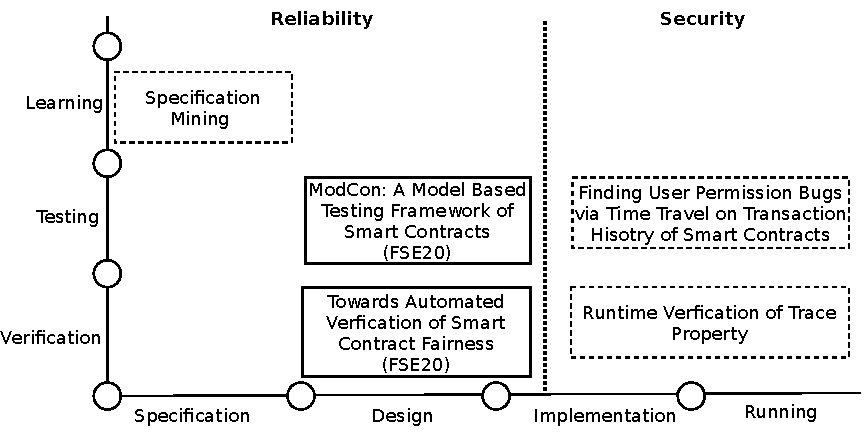
\includegraphics{./Figures/Chapter1/ThesisOverview}
	\caption{The overview of the current work (solid box) and future works (dashed box).}
	\label{fig: thesisoverview}
\end{figure}

To conclude, in this paper, our (future) research aims are threefold:
(1) Ensure smart contract security by performing model based testing for enterprise smart contracts. 
(2) Learn likely specification requirement of smart contracts via time travel on transaction history. 
(3) Verify smart contract fairness of smart contract that reflect the interactions between users and contract.


\section{Main Work and Contribution}
%Our research aims are twofold: (1) ensure smart contract security by performing model based testing for stateful enterprise smart contracts and DApp smart contracts rich in transactions. 
%(2) verify smart contract fairness by modeling users' interaction within smart contract.

\paragraph{Main Work and Contributions}
Our main works and contributions are summarized as follows.
%\yi{Spell out the contributions directly, not through questions.
%For example, what you have designed, proved, implemented, and evaluated.}
%\vspace{-.05in}
\begin{itemize}[leftmargin=*,topsep=4pt]
\item We proposed a general fairness verification framework, \faircon, to check fairness properties of smart contracts.
In particular, we demonstrated \faircon on two types of contracts and four types of fairness properties.
In addition to discovering property violations for bounded models, we apply formal
verification to prove satisfaction of properties for the unbounded cases as well.

\item We designed \modcon allowing users to provide a test model for smart contracts. 
The model is used to specify the state definitions, expected transition relations, pre/post conditions for each transition, invariants, and the mapping from the model to the contract code.
Given the test model, the testing process can also customized by choosing from different coverage strategies and test prioritization options.
\modcon then generates tests with the goal that exercise as many system behaviors as possible while prioritizing on cases of particular interests.

%\item  We proposed a novel approach to apply history transactions for reverse engineering access control models of smart contract. 
%We extracted role-based access control models from history transactions and studied and verified two types of access constraints: (1) separation of duty constraint, and (2) cardinality constraint.
\end{itemize}



\section{Organizations}
The rest of the thesis is organized as follows.
\Cref{ch:preliminary} presents the necessary background about smart contract and blockchain transaction.
The general fairness verification framework, \faircon, will be discussed in \Cref{ch:faircon}.
\Cref{ch:modcon} introduces \modcon, a model-based testing platforms of smart contract.
\Cref{ch:futurework} illustrates our future work, which aims to find permission bugs via time travel on transaction history of smart contracts,
and then this report will be concluded in \Cref{ch:conclusion}.

%\paragraph{Key Terms}
%Smart Contract; Model-based testing; Fairness verification; Program invariant; Automata learning.

%\paragraph{Tip}
%Literature Review; Contribution.